%%%%%%%%%%%%%%%%%%%%%%%% ExtendedAbstract.tex %%%%%%%%%%%%%%%%%%%%%%%%
%                                                                    %
%  Template for the 10-page extended abstract to be submitted for    %
%  the MSc degree conferral at Instituto Superior Tecnico.           %
%                                                                    %
%  Author:                                                           %
%                                                                    %
%       Andre C. Marta                                               %
%       Area Cientifica de Mecanica Aplicada e Aeroespacial          %
%       Departamento de Engenharia Mecanica                          %
%       Instituto Superior Tecnico                                   %
%       Av. Rovisco Pais                                             %
%       1049-001 Lisboa                                              %
%       Portugal                                                     %
%       Tel: +351 21 841 9466                                        %
%                        3466 (extension)                            %
%       Email: andre.marta@ist.utl.pt                                %
%                                                                    %
%  Created:       Dec  2, 2011                                       %
%  Last Modified: Dec 27, 2011                                       %
%%%%%%%%%%%%%%%%%%%%%%%%%%%%%%%%%%%%%%%%%%%%%%%%%%%%%%%%%%%%%%%%%%%%%%
% This document uses the LaTeX class file "article.cls"              %
%%%%%%%%%%%%%%%%%%%%%%%%%%%%%%%%%%%%%%%%%%%%%%%%%%%%%%%%%%%%%%%%%%%%%%
\documentclass[10pt,a4paper,twocolumn]{article}

%%%%%%%%%%%%%%%%%%%%%%%%%%%%%%%%%%%%%%%%%%%%%%%%%%%%%%%%%%%%%%%%%%%%%%
% Document preamble
%%%%%%%%%%%%%%%%%%%%%%%%%%%%%%%%%%%%%%%%%%%%%%%%%%%%%%%%%%%%%%%%%%%%%%

%% Builds upon the graphics  package, providing a key-value interface
%% for optional arguments to the \includegraphics command that go far
%% beyone what the graphics package offers.
%% http://www.ctan.org/tex-archive/help/Catalogue/entries/graphicx.html
%% if you use PostScript figures in your article
%% use the graphics package for simple commands
%% \usepackage{graphics}
%% or use the graphicx package for more complicated commands
%% \usepackage{graphicx}
%% or use the epsfig package if you prefer to use the old commands
%% \usepackage{epsfig}
\usepackage{graphicx} % Enhanced LaTeX Graphics
% Improve double-column float handling and reduce whitespace from floats
% (Avoid extra packages that may be unavailable in the build env)
% Page geometry: tighter margins for better content fit
\usepackage[a4paper,top=15mm,bottom=20mm,left=15mm,right=15mm]{geometry}
% Slightly reduce space between columns
\setlength{\columnsep}{6mm}

% Tighter vertical spacing around floats/captions to avoid large gaps
\setlength{\textfloatsep}{8pt plus 2pt minus 2pt}
\setlength{\dbltextfloatsep}{8pt plus 2pt minus 2pt}
\setlength{\intextsep}{8pt plus 2pt minus 2pt}
\setlength{\abovecaptionskip}{3pt}
\setlength{\belowcaptionskip}{0pt}

% Encourage flexible float placement to reduce unwanted gaps
\renewcommand{\topfraction}{0.95}
\renewcommand{\bottomfraction}{0.85}
\renewcommand{\textfraction}{0.05}
\renewcommand{\floatpagefraction}{0.8}
\renewcommand{\dbltopfraction}{0.95}
\renewcommand{\dblfloatpagefraction}{0.8}

% For colored text
\usepackage{xcolor}

% For clickable URLs
\usepackage{url}

% For professional table rules (toprule, midrule, bottomrule)
\usepackage{booktabs}

% For multirow cells in tables
\usepackage{multirow}

% Multiple figures
\usepackage{subfigure} % subcaptions for subfigures
%\usepackage{subfigmat} % matrices of similar subfigures (not available on this system)

% Declaring new column types
% 'dcolumn' package defines D to be a column specifier with
% three arguments: D{<sep.tex>}{<sep.dvi>}{<decimal places>}
%                  D{<sep.tex>}{<sep.dvi>}{<left digit places>.<right digit places>}
\usepackage{dcolumn}           % decimal-aligned tabular math columns
% d takes a single argument specifying the number of decimal places, e.g., d{2}
% or the number of digits to the left and right of the seperator, e.g., d{3.2}
\newcolumntype{.}   {D{.}{.}{-1}} % column alignedd on the point separator '.'
\newcolumntype{d}[1]{D{.}{.}{#1}} % column centered on the point separator '.'
\newcolumntype{e}   {D{E}{E}{-1}} % column centered on the exponent 'E'
\newcolumntype{E}[1]{D{E}{E}{#1}} % column centered on the exponent 'E'

%% American Mathematical Society (AMS) plain Tex macros
%%
%% The amsmath package is the principal package in the AMS-LaTeX distribution
%% http://www.ctan.org/tex-archive/help/Catalogue/entries/amsmath.html
\usepackage{amsmath}
%%
%% The amsfonts package provides extended TeX fonts
%% http://www.ctan.org/tex-archive/help/Catalogue/entries/amsfonts.html
\usepackage{amsfonts}
%% The amssymb package provides various useful mathematical symbols
\usepackage{amssymb}
%%
%% The amsthm package provides extended theorem environments
%% http://www.ctan.org/tex-archive/help/Catalogue/entries/amsthm.html
\usepackage{amsthm}

%% Improves the interface for defining floating objects such as figures and tables.
%% The package also provides the H float modifier option of the obsolete here package.
%% http://www.ctan.org/tex-archive/help/Catalogue/entries/float.html
\usepackage{float}

%% Control sectional headers. 
%% http://www.ctan.org/tex-archive/help/Catalogue/entries/sectsty.html
\usepackage{sectsty}
%%
%% Redefine the font size of the 'section' and 'subsection' headings
\newcommand{\myFontSize}{\fontsize{11}{0}\selectfont}
\newcommand{\mySubFontSize}{\fontsize{10}{0}\selectfont}
\sectionfont{\myFontSize\bfseries}       % 11pt, Bold face
\subsectionfont{\mySubFontSize\bfseries} % 10pt, Bold face

%% Select alternative section titles.
%% http://www.ctan.org/tex-archive/help/Catalogue/entries/titlesec.html
\usepackage{titlesec}
%%
%% Left indent, before and after spacing
%% (The starred version kills the indentation of the paragraph following the title)
\titlespacing*{\section}{0pt}{12pt}{6pt}
\titlespacing*{\subsection}{0pt}{10pt}{4pt}

%% Section numbers with trailing dots using titlesec (secdot not available)
%% Alternative implementation using titlesec package
\titleformat{\section}{\myFontSize\bfseries}{\thesection.}{1em}{}
\titleformat{\subsection}{\mySubFontSize\bfseries}{\thesubsection.}{1em}{}

% Slightly reduce body font size to improve layout fit
\AtBeginDocument{\small}

% Margins now controlled by geometry; remove manual overrides

% New command to refer to equations as Eq.(1),Eq.(2),...
\newcommand{\eqnref}[1]{Eq.(\ref{#1})}

%%%%%%%%%%%%%%%%%%%%%%%%%%%%%%%%%%%%%%%%%%%%%%%%%%%%%%%%%%%%%%%%%%%%%%%%%%%%%%%%%%%%%%%%
% Title, authors and addresses

\title{Open-Vocabulary Semantic Segmentation of Aerial Photos}
\date{September 2025}
\author{Luis Pedro Soares Marnoto Gaspar Lopes \\ luis.marnoto.gaspar.lopes@tecnico.ulisboa.pt \\ \\ Instituto Superior T\'{e}cnico, Lisboa, Portugal}

%%%%%%%%%%%%%%%%%%%%%%%%%%%%%%%%%%%%%%%%%%%%%%%%%%%%%%%%%%%%%%%%%%%%%%%%%%%%%%%%%%%%%%%%
\begin{document}

% Begin one column section for title and abstract
%
% http://www.faqs.org/faqs/de-tex-faq/part5/
\twocolumn[
\begin{@twocolumnfalse}
\maketitle

%%%%%%%%%%%%%%%%%%%%%%%%%%%%%%%%%%%%%%%%%%%%%%%%%%%%%%%%%%%%%%%%%%%%%%
% ABSTRACT & KEYWORDS
%%%%%%%%%%%%%%%%%%%%%%%%%%%%%%%%%%%%%%%%%%%%%%%%%%%%%%%%%%%%%%%%%%%%%%
%%%%%%%%%%%%%%%%%%%%%%%%%%%%%%%%%%%%%%%%%%%%%%%%%%%%%%%%%%%%%%%%%%%%%%
%     File: ExtendedAbstract_abstr.tex                               %
%     Tex Master: ExtendedAbstract.tex                               %
%%%%%%%%%%%%%%%%%%%%%%%%%%%%%%%%%%%%%%%%%%%%%%%%%%%%%%%%%%%%%%%%%%%%%%

\begin{abstract}

Referring expression segmentation is a fundamental task in computer vision that integrates natural language understanding with precise visual localization of target regions. Applying this to aerial imagery presents unique challenges because spatial resolution varies widely across datasets, targets often shrink to only a few pixels, and scenes contain very high object densities. This work presents Aerial-D, a large-scale referring expression segmentation dataset for aerial imagery comprising 37,288 image patches with 1,522,523 referring expressions covering 259,709 annotated targets across individual objects, groups, and semantic categories spanning 21 distinct classes from vehicles and infrastructure to land cover types. The dataset is constructed through a fully automatic pipeline that combines systematic rule-based expression generation with Large Language Model enhancement, enriching both the linguistic variety and visual detail within the referring expressions. As an additional capability, the pipeline produces dedicated historic counterparts for each scene, supporting real-world archival analyses such as monitoring urban change across decades. A single model is trained on Aerial-D together with prior aerial datasets, yielding unified instance, semantic, and historic segmentation from text, with the historic branch demonstrating robustness to monochrome, sepia, and grainy degradations that appear in archival aerial photography. The dataset, trained models, and complete pipeline are publicly available at \href{https://huggingface.co/datasets/luisml77/aerial-d}{\texttt{huggingface.co/datasets/luisml77/aerial-d}} and \href{https://github.com/luispl77/aerialseg}{\texttt{github.com/luispl77/aerialseg}}.

\vspace{0.3cm}


\end{abstract}


% End one column section (begin default two columns)
\end{@twocolumnfalse}
]
%%%%%%%%%%%%%%%%%%%%%%%%%%%%%%%%%%%%%%%%%%%%%%%%%%%%%%%%%%%%%%%%%%%%%%
% INTRODUCTION
%%%%%%%%%%%%%%%%%%%%%%%%%%%%%%%%%%%%%%%%%%%%%%%%%%%%%%%%%%%%%%%%%%%%%%
%%%%%%%%%%%%%%%%%%%%%%%%%%%%%%%%%%%%%%%%%%%%%%%%%%%%%%%%%%%%%%%%%%%%%%
%     File: ExtendedAbstract_intro.tex                               %
%     Tex Master: ExtendedAbstract.tex                               %
%%%%%%%%%%%%%%%%%%%%%%%%%%%%%%%%%%%%%%%%%%%%%%%%%%%%%%%%%%%%%%%%%%%%%%

\section{Introduction}
\label{sec:intro}

Referring expression segmentation is a computer vision task in which a model receives a natural language description of a target region and must return the corresponding segmentation mask. Because the phrasing can reference any concept, the task is open-vocabulary and the target can be a single instance, a coherent group of instances, or an entire semantic category, such as "all roads in the patch" or "the vegetation strip along the river". The remote-sensing literature coined the term Referring Remote Sensing Instance Segmentation (RRSIS)~\cite{yuan2023rrsis} for the subset that limits expressions to single instances, while later datasets like NWPU-Refer~\cite{yang2024large} incorporated group-level expressions and Aerial-D extends the coverage further to include instances, groups, and full land-cover classes. When this formulation is applied to aerial photographs, although we refer to it simply as referring expression segmentation throughout this article, the problem becomes especially demanding because top-down perspectives compress object scales, spatial resolution varies across sensors, many targets occupy only a handful of pixels, and the scenes themselves contain extreme object densities. In many real deployments, analysts revisit archival aerial surveys to study how cities or coastlines evolved. To support that use case, the pipeline also models the monochrome, sepia, and grainy degradations found in historic imagery so the resulting models can handle tasks such as assessing long-term urban change.

A critical component for developing effective models for RRSIS is access to high-quality datasets containing aerial photographs, precise segmentation masks, and natural referring expressions. To address this need, this work presents Aerial-D, a large-scale referring expression segmentation dataset for aerial imagery comprising 1,522,523 expressions across 37,288 aerial image patches, compared with prior RRSIS datasets~\cite{yuan2023rrsis,liu2024rotated,yang2024large}. Figure~\ref{fig:dataset_examples} highlights how this corpus spans rural and urban scenes and objects, land-cover regions, groups of multiple objects, and entire categories while retaining unrestricted, richly worded referring expressions tailored to each target. Each sample further includes an automatically generated historic counterpart, enabling models trained on the dataset to understand black-and-white, grainy, or sepia aerial imagery alongside contemporary captures.

% Locally tighten spacing for this figure to avoid a visible gap
\begingroup
\setlength{\intextsep}{6pt}
\setlength{\abovecaptionskip}{2pt}
\setlength{\belowcaptionskip}{0pt}
\begin{figure}[H]
\centering
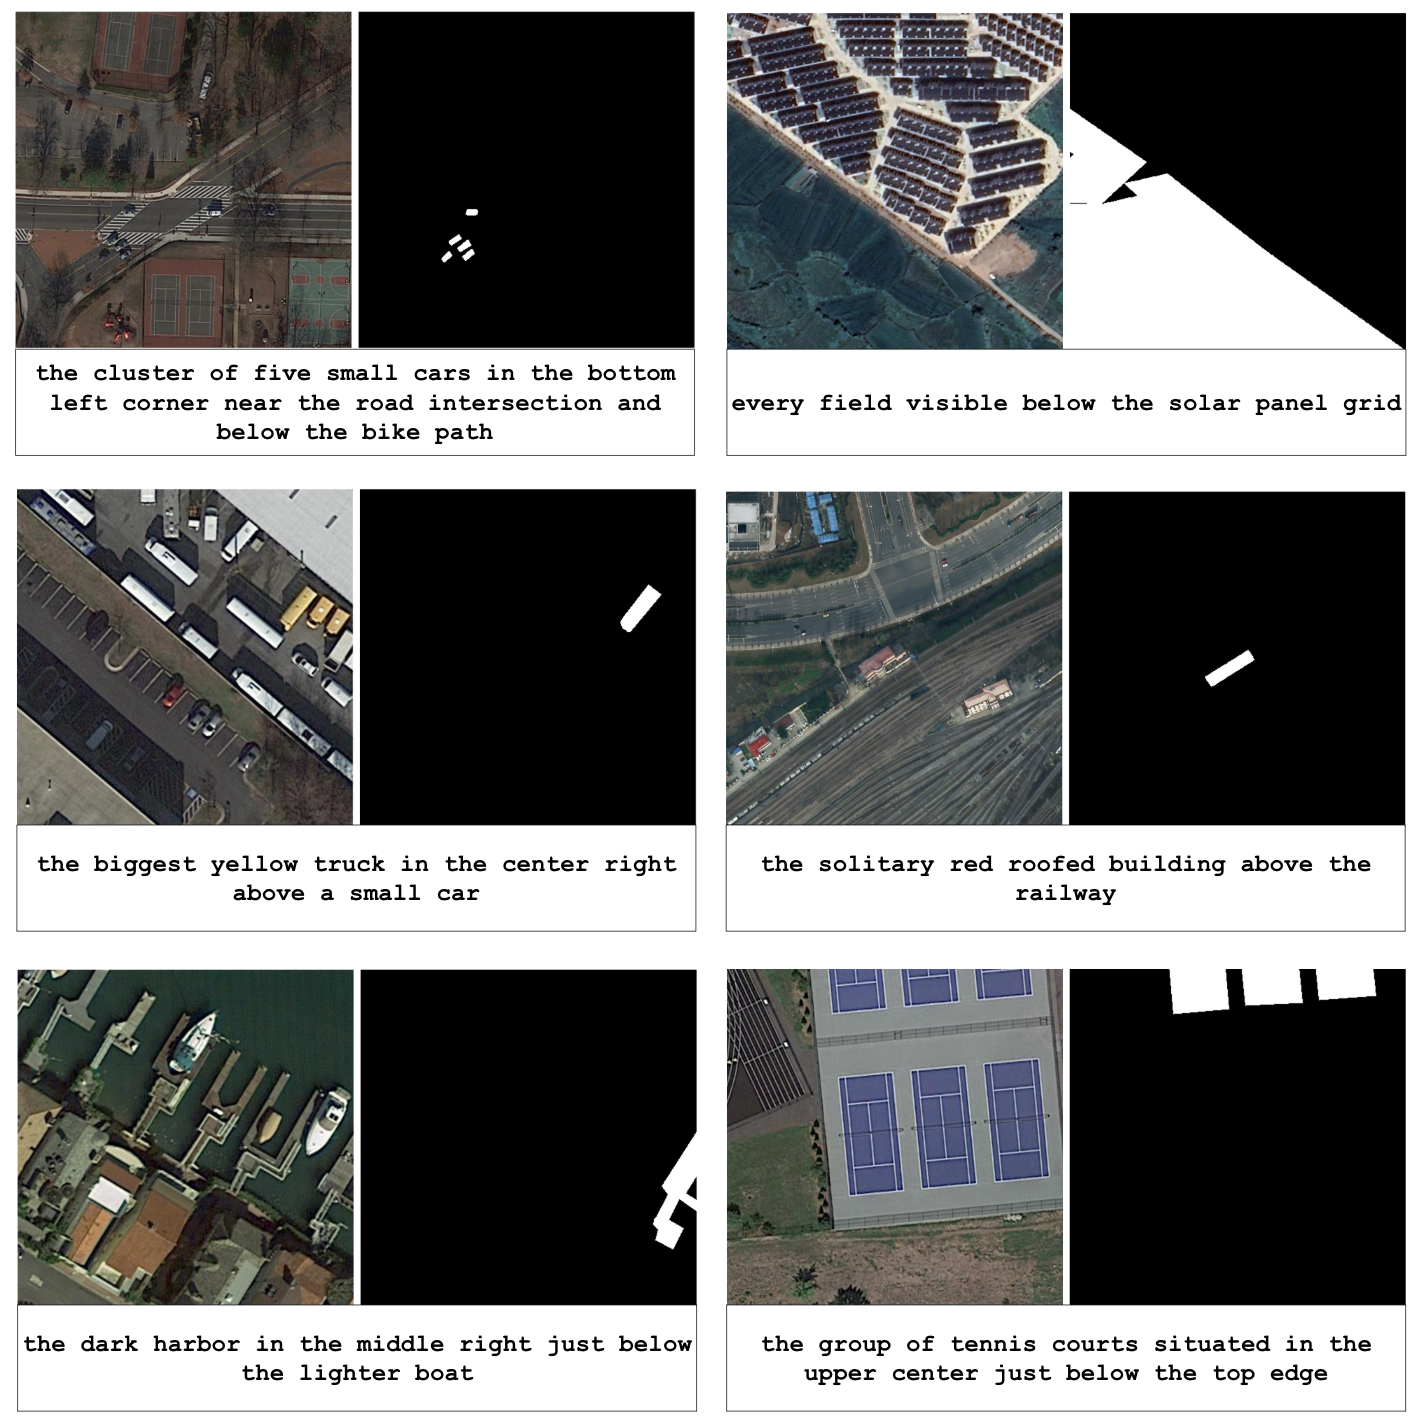
\includegraphics[width=\columnwidth]{./images/6samples.png}
\caption{Representative examples from Aerial-D dataset showing diverse referring expressions with corresponding aerial images and ground truth masks.}
\label{fig:dataset_examples}
\end{figure}
\endgroup


The key contributions of this work include: (1) a comprehensive toolchain that enables the production of complex referring expression datasets from instance segmentation datasets, including a rule-based pipeline, Large Language Model enhancement and distillation methods, and historic image data augmentation with dedicated filtering; (2) the construction of Aerial-D, a dataset comprising over 1.5 million expressions across 37,288 aerial image patches, created entirely through the proposed automatic pipeline; and (3) a unified model trained on Aerial-D alongside four additional datasets, applying the full toolchain—including historic transformations across all training data—to deliver referring expression segmentation over instances, groups, classes, and land cover regions while maintaining reliable performance on degraded historic imagery typical of archival aerial surveys.


%%%%%%%%%%%%%%%%%%%%%%%%%%%%%%%%%%%%%%%%%%%%%%%%%%%%%%%%%%%%%%%%%%%%%%
% RELATED WORK
%%%%%%%%%%%%%%%%%%%%%%%%%%%%%%%%%%%%%%%%%%%%%%%%%%%%%%%%%%%%%%%%%%%%%%
%%%%%%%%%%%%%%%%%%%%%%%%%%%%%%%%%%%%%%%%%%%%%%%%%%%%%%%%%%%%%%%%%%%%%%
%     File: ExtendedAbstract_backg.tex                               %
%     Tex Master: ExtendedAbstract.tex                               %
%%%%%%%%%%%%%%%%%%%%%%%%%%%%%%%%%%%%%%%%%%%%%%%%%%%%%%%%%%%%%%%%%%%%%%

\section{Related Work}
\label{sec:related}

This section reviews the datasets and architectural developments that underpin aerial image understanding, with emphasis on instance and semantic segmentation resources, referring segmentation datasets, historical imagery, and architectures tailored to remote sensing.

\subsection{Aerial Imagery Datasets}

Reliable progress in aerial image understanding depends on datasets that capture both discrete objects (e.g., ships, vehicles) and continuous land cover (e.g., roads, water, vegetation), as well as benchmarks that test language-based selection of specific targets. We first summarize instance and semantic segmentation resources that established pixel-level ground truth, and then discuss the emergence of referring segmentation datasets that couple images, masks, and natural language.

\subsubsection{Instance and Semantic Segmentation}

The iSAID dataset~\cite{zamir2019isaid} established the foundation for instance segmentation in aerial imagery by providing 655,451 object instances across 15 categories in 2,806 high-resolution images. Building upon the DOTA dataset, iSAID addressed the unique challenges of aerial imagery including high object density, large scale variations, and arbitrary orientations. The dataset demonstrated that existing computer vision methods require specialized adaptation for aerial domains, as off-the-shelf approaches achieved suboptimal performance.

Complementing instance-level analysis, the LoveDA dataset~\cite{wang2021loveda} focused on land-cover semantic segmentation across urban and rural environments. Covering 536.15 km² with 0.3m resolution imagery, LoveDA enables domain adaptation research by addressing style differences between geographical environments, with urban scenes dominated by artificial objects and rural scenes containing natural elements.

\subsubsection{Referring Segmentation Datasets}

While instance and semantic segmentation establish pixel-accurate supervision, they assume a fixed label set. Referring segmentation reframes the problem: given a natural language phrase, the goal is to select and segment the specific object (or group) described. In aerial imagery, this line of work began with RefSegRS~\cite{yuan2023rrsis}, which introduced 4,420 image–language–mask triplets and formalized Referring Remote Sensing Instance Segmentation (RRSIS). The dataset highlighted aerial-specific challenges—small, densely packed targets and cluttered layouts—where language can disambiguate between visually similar instances.

RRSIS-D~\cite{liu2024rotated} expanded both scale and annotation efficiency with 17,402 image–caption–mask triplets generated through a semi-automated pipeline using the Segment Anything Model (SAM). Beyond size, it targets aerial-specific phenomena—broad spatial scales and diverse object orientations—across 20 categories and seven attribute dimensions, enabling richer evaluation of language-guided selection in overhead scenes.

NWPU-Refer~\cite{yang2024large} further broadens coverage with 15,003 high-resolution images and 49,745 annotated targets spanning more than 30 countries. In contrast to semi-automated pipelines, it emphasizes purely manual annotation quality and explicitly supports single-object, multi-object, and non-object scenarios across 32 categories. Together, these benchmarks trace a steady shift from fixed-category segmentation toward language-conditioned, fine-grained selection in aerial imagery.

\subsubsection{Historical Imagery Applications}

Analysing historical aerial photographs introduces practical complications—reduced contrast, grayscale capture, film artifacts, and geometric distortions—yet these datasets are vital for studying long-term urban change. Urban1960SatSeg~\cite{hao2025urban1960satseg} addresses this gap with professionally annotated semantic segmentation over 1,240 km² of declassified mid-20th-century imagery from Xi'an, China. By focusing on degraded visual conditions, it provides a reference point for methods that must remain robust when applied to archival aerial data.

\subsection{Architectures for RRSIS}

Architectures for referring segmentation in aerial imagery follow two broad paths. One family builds specialized networks tailored to overhead scenes, emphasizing multi-scale fusion and rotation handling without relying on large vision–language backbones. A second family leverages foundation models—vision encoders (e.g., CLIP or SigLIP) and segmentation decoders (e.g., SAM)—and focuses on bridging text–vision semantics for mask prediction. We outline representative approaches from both lines of work.

The Rotated Multi-Scale Interaction Network (RMSIN)~\cite{liu2024rotated} exemplifies the specialized-network path. It introduces three modules—Intra-scale Interaction (IIM) for fine-grained detail, Cross-scale Interaction (CIM) for multi-resolution fusion, and Adaptive Rotated Convolution (ARC) for orientation variation—achieving improvements over strong baselines and showing the value of remote-sensing-specific inductive biases.

RSRefSeg~\cite{chen2025rsrefseg} represents the foundation-model path: it couples a vision–language encoder (CLIP) with a segmentation decoder (SAM) and learns a bridge mechanism (AttnPrompter) that converts text semantics into decoder-friendly prompts. With parameter-efficient fine-tuning (e.g., LoRA), this design achieves strong performance while reusing powerful pretraining. Figure~\ref{fig:rsrefseg_arch} illustrates this foundation-model architecture for referring segmentation in aerial imagery.

MRSNet~\cite{yang2024large} advances the specialized-network line with intra-scale and hierarchical feature interaction modules designed to better capture multi-scale context in overhead scenes. In contrast, foundation-model approaches emphasize powerful pretrained backbones and light semantic bridging, trading bespoke inductive biases for transfer from large-scale pretraining.

\begin{figure*}[t]
\centering
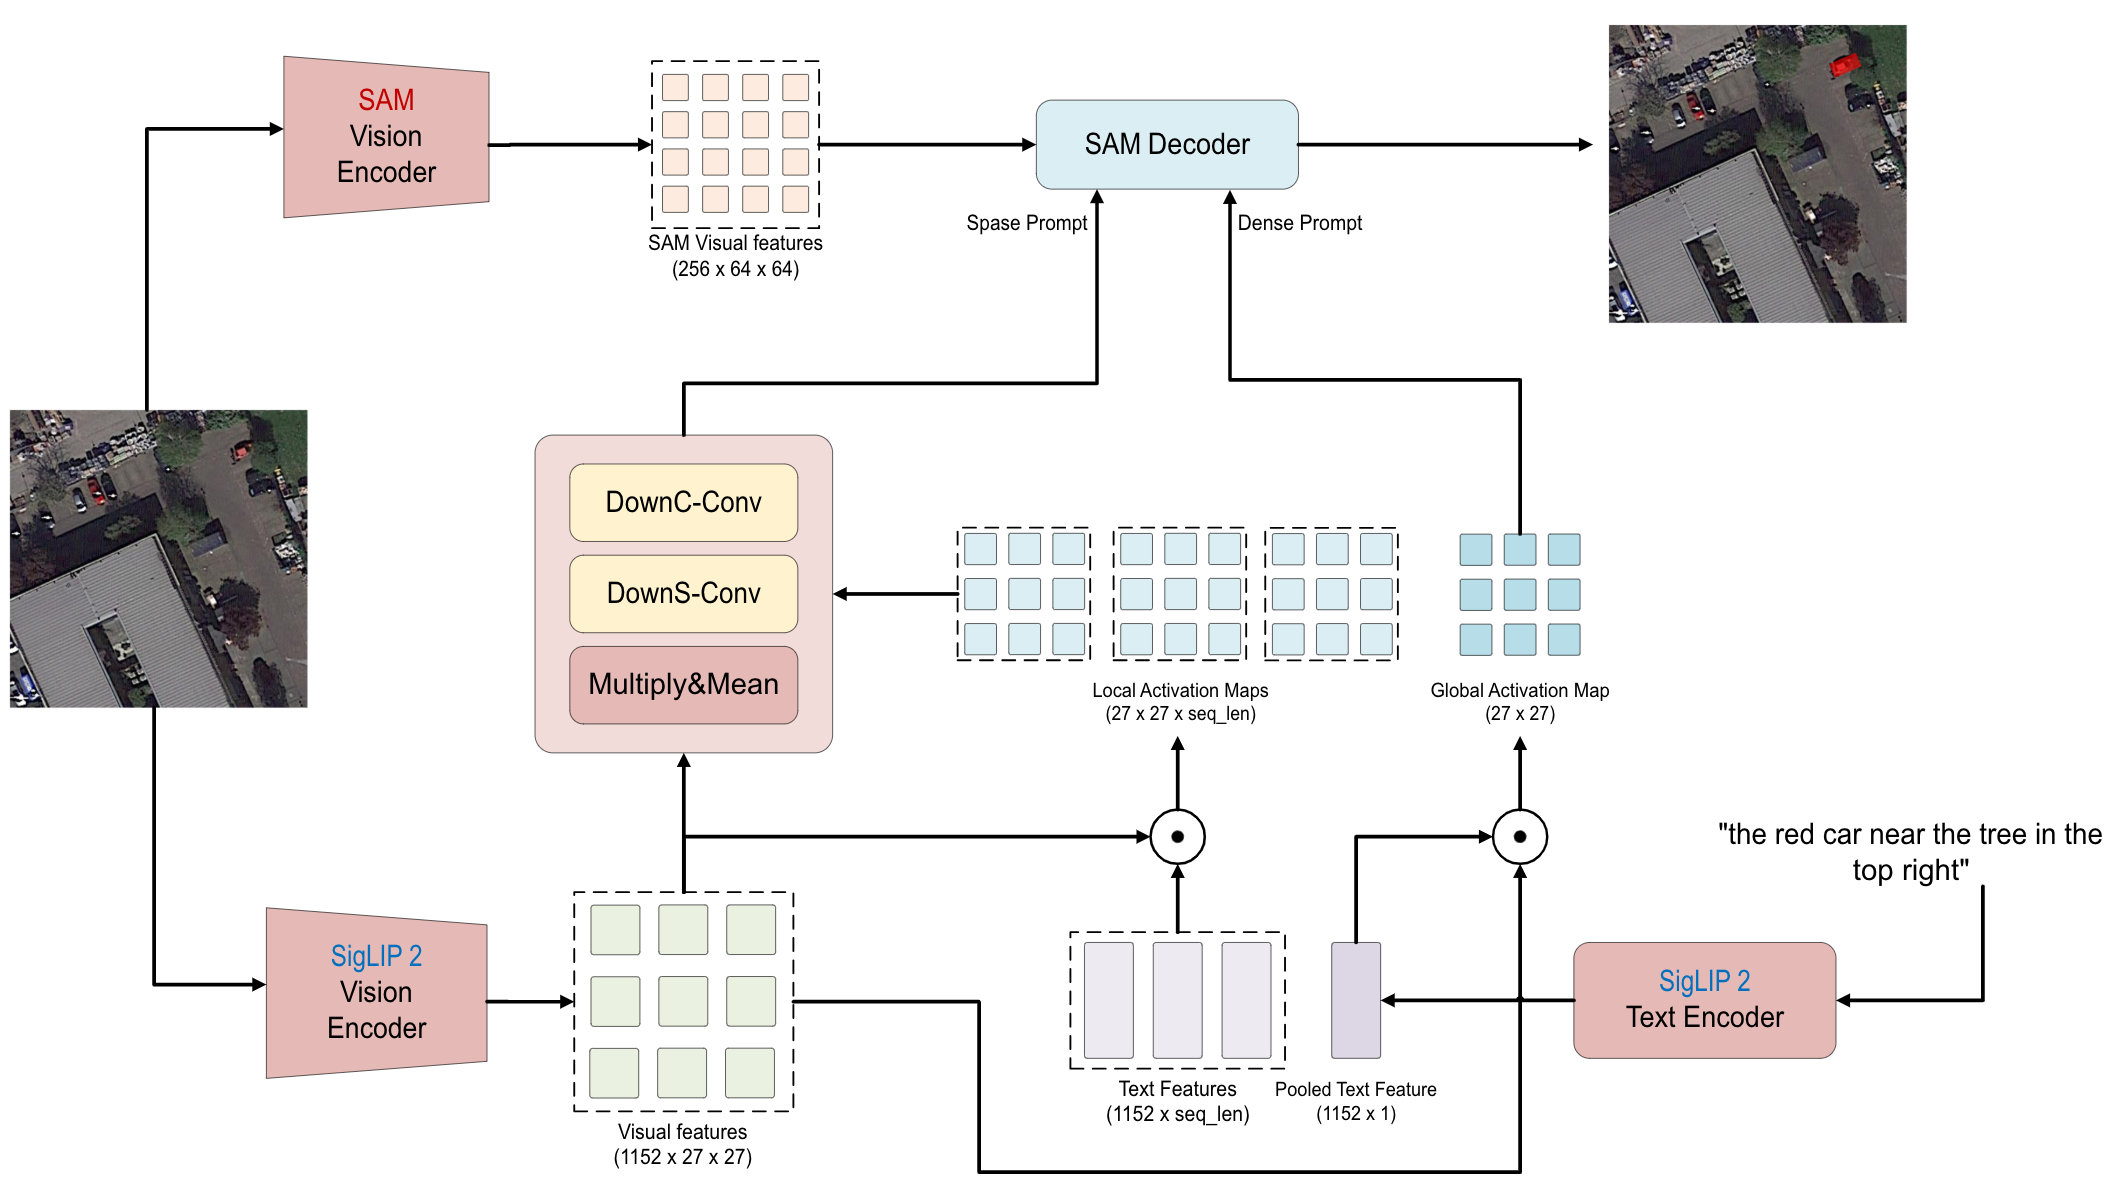
\includegraphics[width=0.9\textwidth]{./images/rsrefseg.png}
\caption{Overview of the RSRefSeg architecture~\cite{chen2025rsrefseg}, which couples a vision–language encoder with a segmentation decoder via a learned prompting bridge; a representative example of foundation-model approaches to aerial referring segmentation.}
\label{fig:rsrefseg_arch}
\end{figure*}

\subsection{Overview}

The current landscape provides three pillars for language-guided segmentation in aerial imagery. First, instance and semantic datasets such as iSAID and LoveDA supply pixel-accurate supervision for objects and land cover. Second, referring segmentation benchmarks including RefSegRS, RRSIS-D, and NWPU-Refer pair images with natural expressions and masks, enabling evaluation of language-conditioned target selection at varying scales and annotation regimes. Third, architectural developments span specialized remote-sensing networks (e.g., RMSIN, MRSNet) and foundation-model designs (e.g., RSRefSeg) that leverage strong vision and language backbones.

Crucially, the complementary supervision in iSAID and LoveDA presents an opportunity to construct a larger and more diverse referring segmentation resource by converting instance- and land-cover annotations into language-conditioned targets—motivating the creation of Aerial-D as a comprehensive benchmark for aerial referring expressions.

Within this context, RSRefSeg stands out as a particularly compelling choice for referring expression segmentation: it benefits from powerful pretrained vision–language encoders (e.g., CLIP/SigLIP) and a high-capacity segmentation decoder (SAM), connected by a lightweight bridging mechanism. This combination offers strong generalization with modest task-specific adaptation, making it a natural starting point for modern aerial referring segmentation systems.


%%%%%%%%%%%%%%%%%%%%%%%%%%%%%%%%%%%%%%%%%%%%%%%%%%%%%%%%%%%%%%%%%%%%%%
% APPROACH FOR DATASET GENERATION
%%%%%%%%%%%%%%%%%%%%%%%%%%%%%%%%%%%%%%%%%%%%%%%%%%%%%%%%%%%%%%%%%%%%%%
%%%%%%%%%%%%%%%%%%%%%%%%%%%%%%%%%%%%%%%%%%%%%%%%%%%%%%%%%%%%%%%%%%%%%%
%     File: ExtendedAbstract_imple.tex                               %
%     Tex Master: ExtendedAbstract.tex                               %
%%%%%%%%%%%%%%%%%%%%%%%%%%%%%%%%%%%%%%%%%%%%%%%%%%%%%%%%%%%%%%%%%%%%%%

\section{Aerial-D Dataset Construction}
\label{sec:approach}

This section details our comprehensive approach to constructing Aerial-D, a large-scale referring expression segmentation dataset for aerial imagery. Our methodology combines automated rule-based expression generation with large language model enhancement to achieve both scale and linguistic diversity. We begin by establishing our source datasets, then describe our rule-based pipeline for generating referring expressions from existing annotations, followed by our novel knowledge distillation approach for cost-effective LLM enhancement, and conclude with comprehensive dataset statistics demonstrating the scope and characteristics of the final resource.

\subsection{Source Datasets}

The Aerial-D dataset is constructed from two complementary aerial datasets with different annotation styles: iSAID (instance segmentation) and LoveDA (semantic segmentation).

We start by putting both sources into the same format so that a single model can learn from them side by side: square patches at 480×480. This size keeps small iSAID objects large enough to describe and segment, while fitting the input expectations of common vision encoders used in our model (e.g., CLIP/SigLIP image towers and SAM backbones\cite{clip,siglip,sam}).

From there, preparation is straightforward. For iSAID’s very large images, we use an overlapping sliding window and keep the patches that contain valid instances. For LoveDA, we resize to the same patch size and derive instance targets for the classes of interest—buildings and water—using connected-component analysis on the semantic masks. We also retain the full semantic labels per patch. Buildings and water are amenable to instance-level treatment; while water is a land-cover class, in LoveDA it predominantly appears as well-defined lakes and some rivers, which people naturally refer to as discrete entities or sets. Other land-cover classes (e.g., farmland or forest) behave as continuous surfaces, so splitting them into arbitrary components would create unnatural targets for referring expressions. We therefore keep those land-cover classes at the category level with encompassing descriptions, while promoting buildings and water to instance targets. The result is a unified per-patch representation with instance targets and complete category labels, which we then use for rule-guided expression generation.

\subsection{Rule-Based Expression Generation}

The core challenge is figuring out how to describe these target objects using only what we know from their bounding boxes, masks, and categories. We utilize the bounding box coordinates to understand where each object sits within the image patch. As shown in Figure \ref{fig:rule_example}, we divide each patch into a three-by-three grid marked with dotted lines, so we can say an object is "in the top right" or "in the center". When we have multiple objects of the same type, we also check if any are in extreme positions like the topmost or leftmost instance of that category.

Since we also have the pixel masks for each object, we can analyze their colors by looking at HSV values to distinguish between light and dark objects, and various chromatic colors. However, we avoid using color descriptions for buildings and water since these typically show mixed colors that aren't useful for identification.

We also create relationships between nearby objects by calculating angles between their positions, allowing us to generate expressions like "the ship to the left of the harbor" or "the vehicle above the building". The system uses eight directional relationships: above, below, to the left of, to the right of, and the four diagonal directions.

All these rules combine to generate various referring expressions for each object, as demonstrated in Figure \ref{fig:rule_example} where a single plane generates multiple possible descriptions including "the plane in the top right", "the light plane in the top right", and versions with relational descriptions. However, a significant challenge emerges when multiple objects end up with identical characteristics and generate the exact same expressions, creating ambiguous references where one phrase could describe multiple different objects. We solve this fundamental problem by taking the set of all expressions for all objects and targets in each image, matching them against each other to find duplicates, and when we find expressions that are identical, we cancel both expressions out and discard them as ambiguous. This ensures every remaining phrase points to exactly one target.

\begin{figure*}[t]
\centering
\begin{minipage}{0.5\textwidth}
\centering
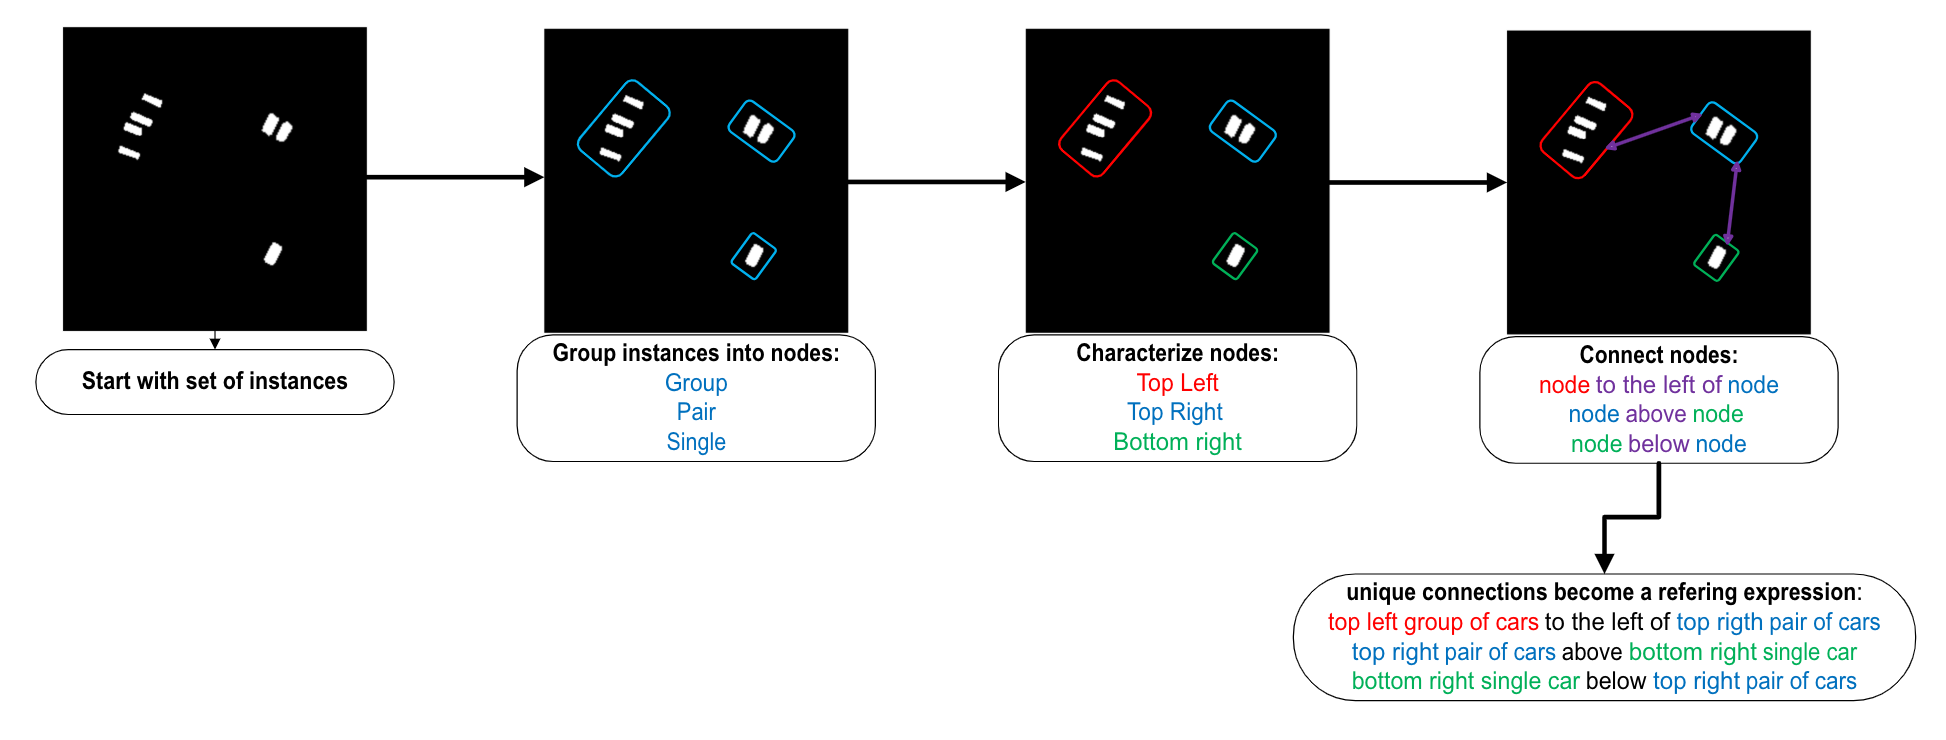
\includegraphics[width=0.65\textwidth]{./images/rule_based_generation.png}
\end{minipage}%
\begin{minipage}{0.5\textwidth}
\centering
\hspace{-1cm}
\raisebox{-0.3\height}{%
\resizebox{\textwidth}{!}{%
\footnotesize
\begin{tabular}{@{}ll@{}}
\toprule
\textbf{Rule Type} & \textbf{Example Instance} \\
\midrule
Category & "plane" \\
Grid Position & "in the top right" \\
Extreme Position & None \\
Color Classification & "light" \\
Directional Relations & "to the bottom right of a plane" \\
& "to the top right of a plane" \\
\midrule
\multicolumn{2}{l}{\textbf{Final Expressions}} \\
\multicolumn{2}{l}{"the plane in the top right"} \\
\multicolumn{2}{l}{"the light plane in the top right"} \\
\multicolumn{2}{l}{"the plane in the top right to the bottom right of a plane"} \\
\multicolumn{2}{l}{"the light plane in the top right to the bottom right of a plane"} \\
\multicolumn{2}{l}{"the plane in the top right to the top right of a plane"} \\
\multicolumn{2}{l}{"the light plane in the top right to the top right of a plane"} \\
\bottomrule
\end{tabular}%
}%
}

\end{minipage}
\caption{Example of rule generation for a single instance. The highlighted plane in the top right section demonstrates how the system assigns spatial, visual, and relational rules that will later be combined into referring expressions.}
\label{fig:rule_example}
\end{figure*}


\subsection{LLM Expression Generation}
\label{subsec:llm_expression_generation}
While rule-based expression generation provides a solid foundation for referring expression data, these expressions suffer from significant limitations in language variation and visual detail coverage. The rule-based approach produces linguistically constrained expressions with limited wording variations and lacks the ability to reference contextual elements beyond predefined source dataset categories.

To address these limitations, we employ a multimodal Large Language Model (LLM) to enhance our dataset by providing both images and expressions as input, enabling the model to rewrite and improve the original referring expressions. We target enhancement from two approaches, as shown in Figure \ref{fig:llm_enhancement_example}. The first approach focuses on linguistic variation, creating natural language alternatives for each rule-based expression without heavy reliance on visual information. The second approach uses visual information, where the model examines surrounding features in the image around the target object. We provide bounding box annotations to help the model focus on the correct target region, as demonstrated in Figure \ref{fig:llm_enhancement_example} with the group of large vehicles.

This dual approach transforms basic expressions like "the group of 4 large vehicles in the top center" into linguistically diverse alternatives such as "the cluster of four big vehicles near the upper middle" and visually detailed descriptions like "the four large vehicles lined up side by side just below the pale paved strip at the very top middle", where the model identifies and references contextual elements not captured in the original datasets, such as the "pale paved strip" and the "grassy area".

However, the full dataset contains approximately 300,000 captured targets including both objects and groups. To generate expressions, we process each target individually, meaning we would need 300,000 separate LLM requests. Using production-grade LLMs at this scale—for example, OpenAI’s o3 model\cite{o3} with strong visual capabilities—would cost thousands of dollars; Table \ref{tab:cost_comparison} reports the exact breakdown, making direct application prohibitively expensive for research-scale dataset construction.

To address this scalability challenge, we employ a knowledge distillation approach, as illustrated in Figure \ref{fig:llm_distillation}. We utilize OpenAI’s o3 model\cite{o3} and compare it against a much more lightweight open‑weights model, Gemma3\cite{gemma3}. We obtain 500 high‑quality outputs from o3 on a representative random subset of targets from the initial dataset. These outputs serve as training data for supervised fine‑tuning using the parameter‑efficient QLoRA method\cite{qlora} on Gemma3‑12B.

The custom‑tailored fine‑tuned Gemma3 model can then process all 300,000 targets using a single GPU, resulting in a much cheaper and more efficient method. Notably, the distilled model’s output quality approaches o3’s once fine‑tuned; qualitative comparisons in Figure \ref{fig:distillation_comparison} show closely matched enhancements with markedly reduced hallucinations relative to the base Gemma3 model.

\begin{figure*}[t]
\centering
\begin{minipage}{0.5\textwidth}
\centering
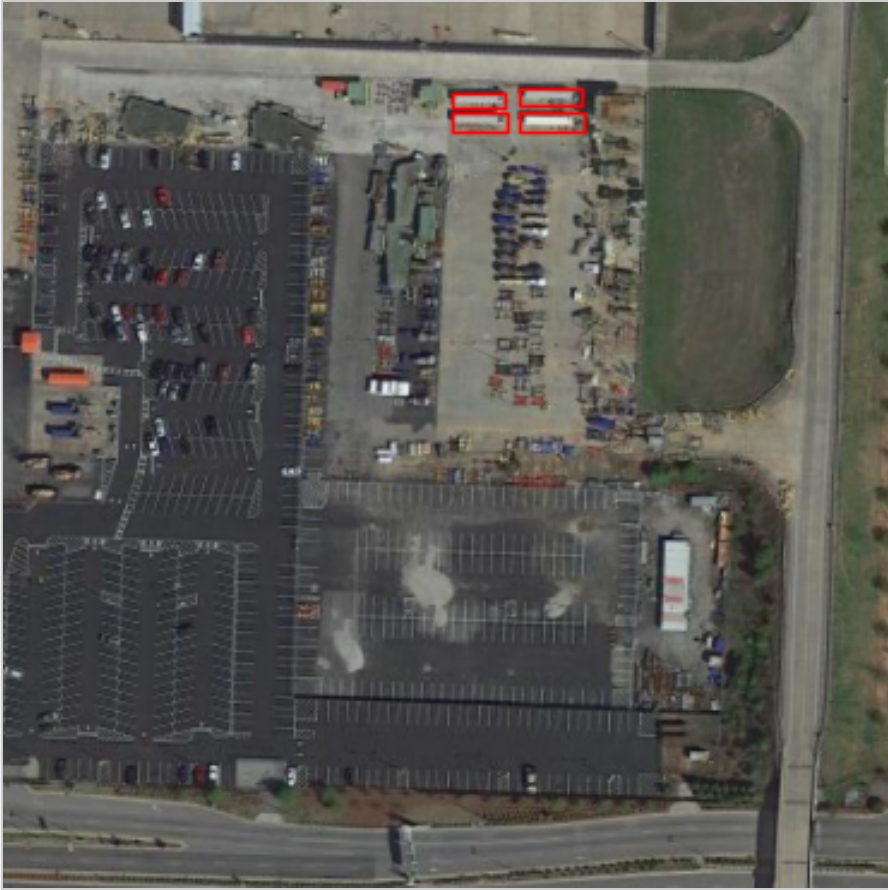
\includegraphics[width=0.65\textwidth]{./images/example_group.png}
\end{minipage}%
\begin{minipage}{0.5\textwidth}
\centering
\hspace{-1cm}
\raisebox{-0.3\height}{%
\footnotesize
\begin{tabular}{@{}p{2cm}p{5cm}@{}}
\toprule
\textbf{Expression Type} & \textbf{Example} \\
\midrule
Original & the group of 4 large vehicles in the top center \\
\midrule
Enhanced & the cluster of four big vehicles near the upper middle \\
\midrule
Unique & the four large vehicles lined up side by side just below the pale paved strip at the very top middle \\
\midrule
Unique & the set of four big vehicles parked in a single row in the upper center beside the grassy area to the right \\
\bottomrule
\end{tabular}%
}
\end{minipage}
\caption{Example of LLM enhancement process showing original aerial image with group of four large vehicles (left) and corresponding expression enhancements (right).}
\label{fig:llm_enhancement_example}
\end{figure*}


% (moved later to improve float ordering and reduce gaps)

\subsection{Historic Image Filter Augmentation}
\label{subsec:historic_filters}

In order to improve robustness to archival image conditions, we augment training with three parametric transformations that reproduce characteristic degradations of historical aerial photographs: monochrome capture, contrast roll‑off with film grain, and sepia toning with scan noise (see Figure~\ref{fig:historic_filters}). 

Let $I_{orig}(x)\in[0,255]^3$ denote the RGB image at pixel $x$, and let $\operatorname{clip}(\cdot)$ clamp values to $[0,255]$.

We simulate grayscale capture by converting to luminance, as in \eqnref{eq:gray}:
\begin{equation}
I_{\text{bw}}(x) = 0.299\,R(x) + 0.587\,G(x) + 0.114\,B(x).
\label{eq:gray}
\end{equation}

To emulate film response and grain, we first apply a mild gamma adjustment (\eqnref{eq:gamma}), then a linear contrast change around the mean (\eqnref{eq:contrast}), followed by additive Gaussian noise (\eqnref{eq:grain}):
\begin{equation}
I_{\gamma}(x) = 255\,\big(I_{\text{bw}}(x)/255\big)^{\gamma}.
\label{eq:gamma}
\end{equation}
\begin{equation}
I_{c}(x) = \big(I_{\gamma}(x) - \mu\big)\,c + \mu.
\label{eq:contrast}
\end{equation}
\begin{equation}
I_{\text{grain}}(x) = \operatorname{clip}\big(I_{c}(x) + \eta(x)\big),\quad \eta(x)\sim\mathcal{N}(0,\sigma^2).
\label{eq:grain}
\end{equation}
We use $\gamma=1.1$, $c=0.85$, and $\sigma=0.1\times 255$ to produce mild contrast loss and film grain.

Finally, we apply a fixed sepia transform (\eqnref{eq:sepia}) followed by uniform sensor/scan noise (\eqnref{eq:sepia_noise}):
\begin{equation}
\begin{bmatrix} S_R(x) \\ S_G(x) \\ S_B(x) \end{bmatrix}
= \operatorname{clip}\left(
\begin{bmatrix}
0.272 & 0.534 & 0.131 \\
0.349 & 0.686 & 0.168 \\
0.393 & 0.769 & 0.189
\end{bmatrix}
\begin{bmatrix} R(x) \\ G(x) \\ B(x) \end{bmatrix}
\right).
\label{eq:sepia}
\end{equation}
\begin{equation}
I_{\text{sepia}}(x) = \operatorname{clip}\big(\mathbf{S}(x) + \xi(x)\big),\quad \xi(x)\sim\mathcal{U}(0,50).
\label{eq:sepia_noise}
\end{equation}

These effects mimic tonal range reduction and graininess typical of mid‑century aerial photography while preserving the spatial structure that segmentation relies on. Figure~\ref{fig:historic_filters} illustrates the visual impact of each transformation.

\begin{figure*}[t]
\centering
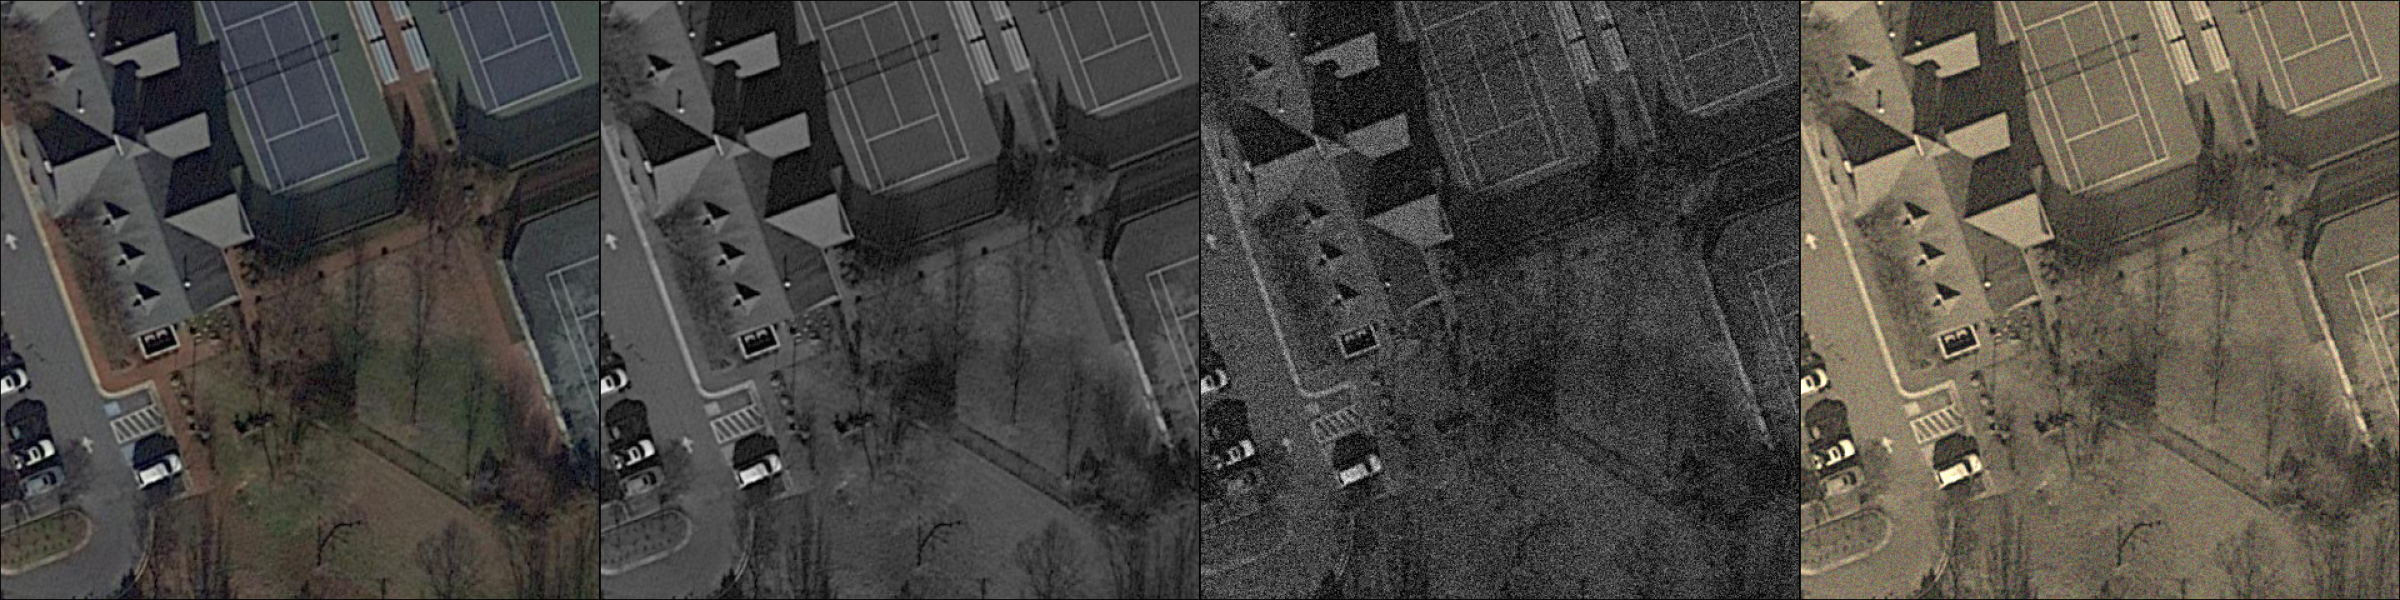
\includegraphics[width=0.9\textwidth]{./images/filters.png}
\caption{Comparison of original aerial image patch with three historic filter transformations: grayscale conversion, sepia toning, and Gaussian noise addition. These filters simulate common degradation patterns in historical aerial photography.}
\label{fig:historic_filters}
\end{figure*}

\subsection{Final Dataset Statistics}

The rule-based generation yields 506{,}194 starting expressions and identifies 259{,}709 annotated targets across the corpus (Table~\ref{tab:llm_enhancement_stats}). Building on this base, the LLM enhancement is prompted to produce one language variation for each original expression and two unique visual-detail expressions for each target, adding 496{,}895 and 519{,}434 expressions respectively and resulting in 1{,}522{,}523 total expressions. Figure~\ref{fig:expression_wordcloud} illustrates how this process expands the vocabulary, as shown in the word cloud.


\begin{figure}[!t]
\centering
\includegraphics[width=\columnwidth]{./images/expression_wordcloud.png}
\caption{Word cloud visualization of the most frequent terms in Aerial-D referring expressions, highlighting the domain-specific vocabulary and spatial descriptors characteristic of aerial imagery.}
\label{fig:expression_wordcloud}
\end{figure}

\begin{figure*}[t]
\centering
\begin{minipage}{0.48\textwidth}
\centering
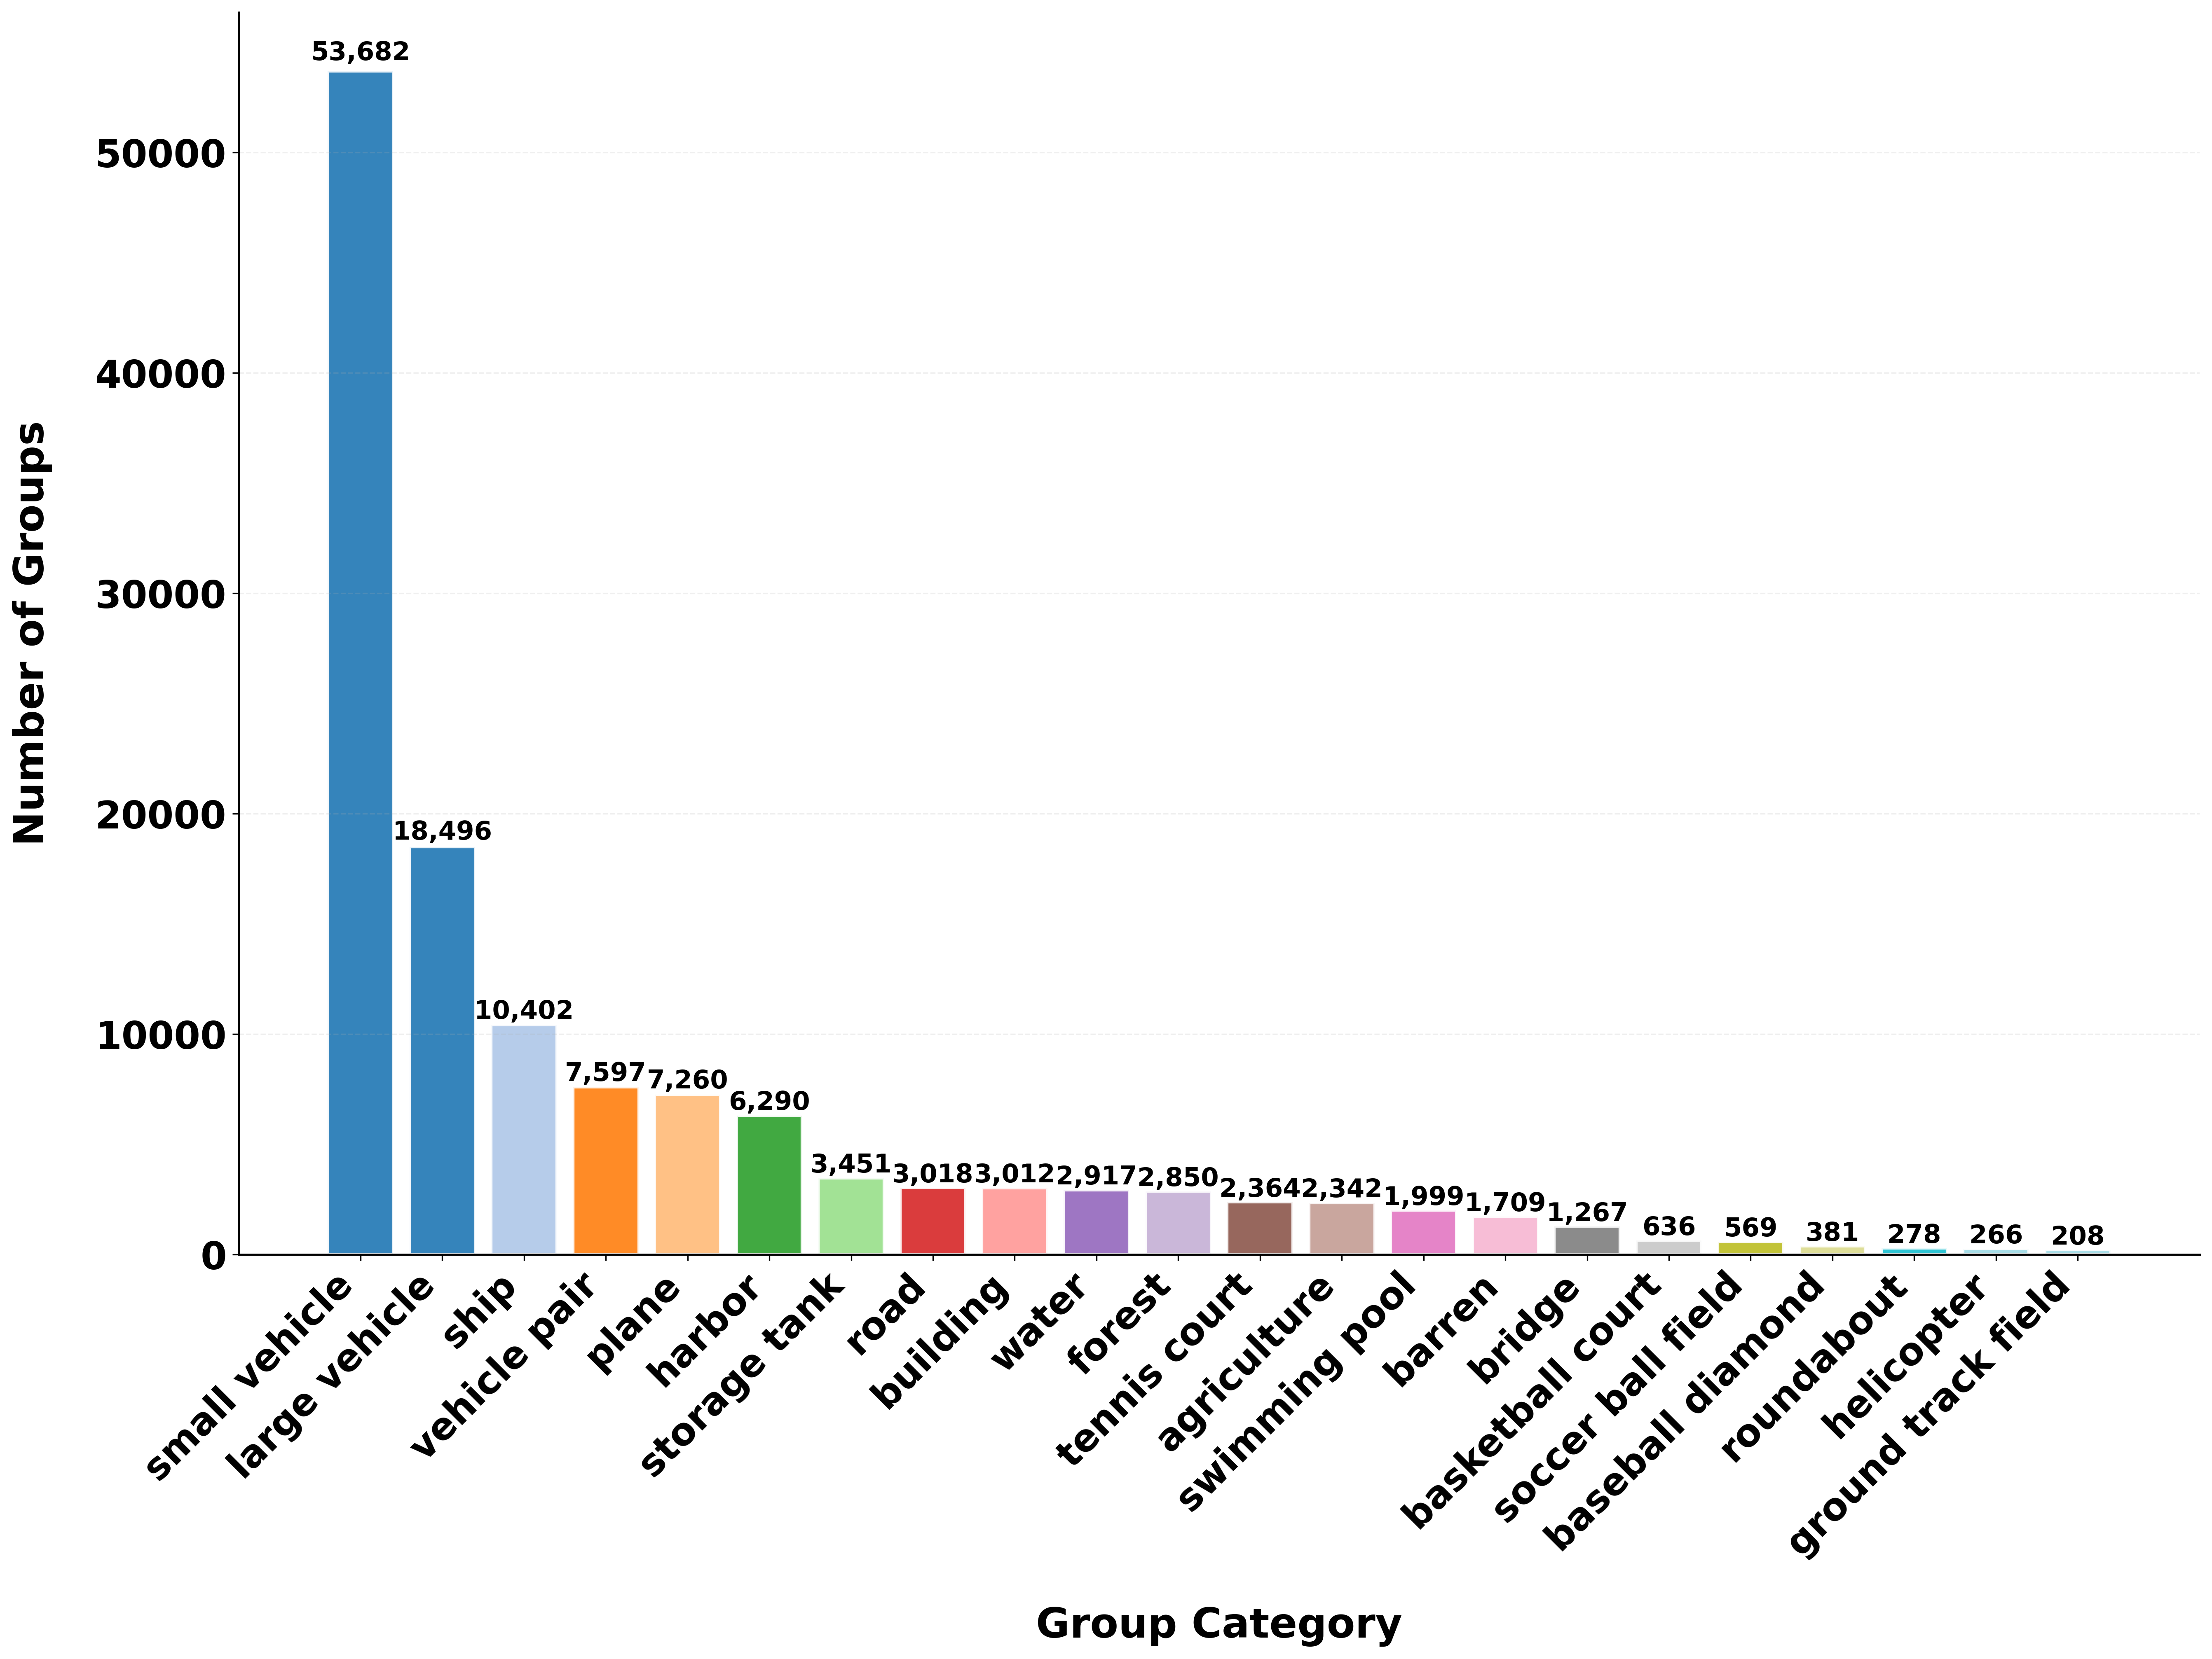
\includegraphics[width=\textwidth]{./images/group_category_distribution.png}
\end{minipage}\hfill
\begin{minipage}{0.48\textwidth}
\centering
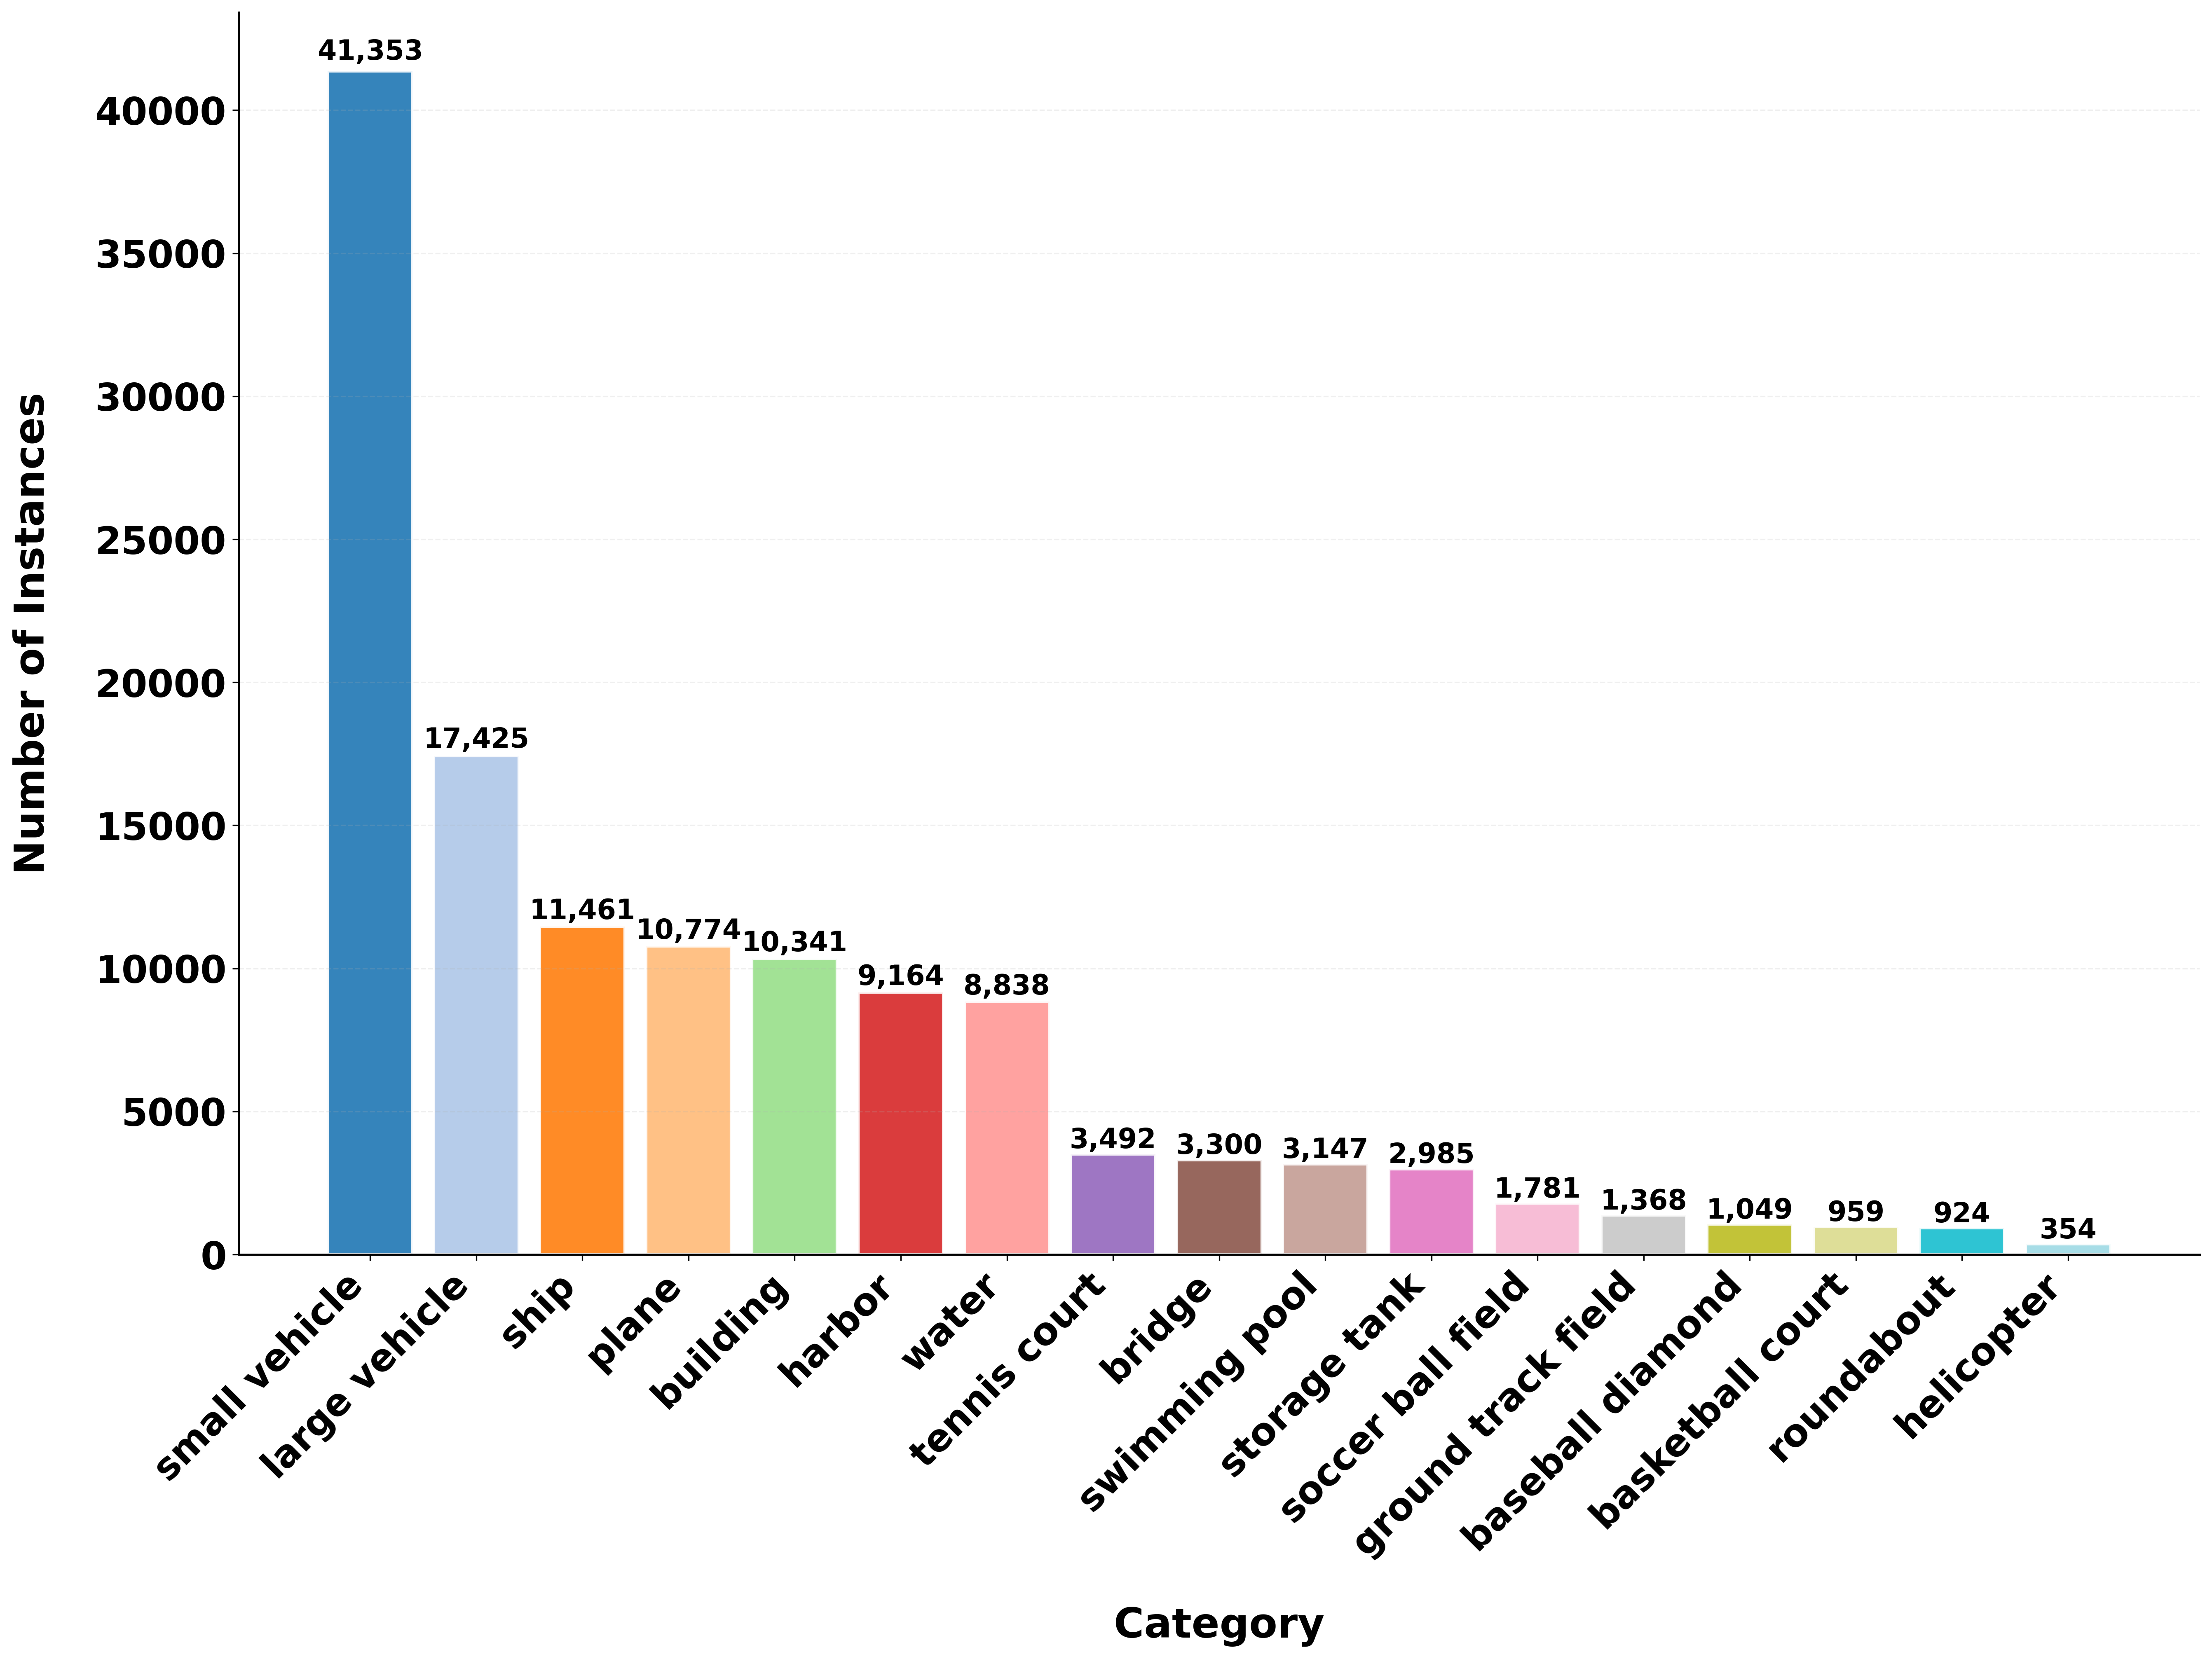
\includegraphics[width=\textwidth]{./images/instance_category_distribution.png}
\end{minipage}
\caption{Category distribution analysis of Aerial-D dataset. Left: Distribution of group annotations showing the prevalence of different object categories in group-level referring expressions. Right: Distribution of individual instance annotations across semantic categories, demonstrating the dataset's coverage of aerial object types.}
\label{fig:category_distributions}
\end{figure*}


Table~\ref{tab:dataset_comparison} compares Aerial-D with prior RRSIS datasets and shows how it scales along three axes: images, targets per image, and expressions per target. First, Aerial-D contains nearly three times as many images as previous datasets. Second, each image typically includes many segmented targets. Third, each target is paired with multiple referring expressions. Together, these factors yield more than 1.5 million referring expressions, positioning Aerial-D among the largest publicly available RRSIS resources. Beyond scale, Aerial-D relies on a fully automatic pipeline that combines rule-based generation with LLM enhancement and supports both single-object and multi-object references. Figure~\ref{fig:category_distributions} breaks down how frequently each semantic category appears at the group and instance levels, confirming that vehicles, buildings, and infrastructure dominate the long tail and that the augmentation strategy preserves the original category balance.

% Dataset comparison table
\begin{table*}[t]
\centering
\caption{Comparison with Existing RRSIS Datasets}
\label{tab:dataset_comparison}
\resizebox{\textwidth}{!}{%
\begin{tabular}{@{}lcccccccc@{}}
\toprule
\textbf{Dataset} & \textbf{Image Resolution} & \textbf{Images} & \textbf{Instance Expr.} & \textbf{Semantic Expr.} & \textbf{Single-object} & \textbf{Multi-object} & \textbf{Patch Size} & \textbf{Annotation Generation} \\
\midrule
RefSegRS & 0.13m & 4,420 & 4,420 & -- & \checkmark & $\times$ & 512 & Manual \\
RRSIS-D & 0.5m-30m & 17,402 & 17,402 & -- & \checkmark & $\times$ & 800 & Semi-auto \\
NWPU-Refer & 0.12m-0.5m & 15,003 & 49,745 & -- & \checkmark & \checkmark & 1,024-2,048 & Manual \\
\midrule
\multirow{2}{*}{\textbf{AERIAL-D}} & \multirow{2}{*}{\textbf{0.3m-4.5m}} & \multirow{2}{*}{\textbf{37,288}} & \textbf{1,278,453} & -- & \textbf{\checkmark} & \textbf{\checkmark} & \multirow{2}{*}{\textbf{480}} & \multirow{2}{*}{\textbf{Automated + LLM}} \\
 & & & -- & \textbf{244,070} & $\times$ & \textbf{\checkmark} & & \\
\bottomrule
\end{tabular}%
}
\end{table*}

\begin{table}[t]
\centering
\caption{Expression Distribution by Source}
\label{tab:llm_enhancement_stats}
\footnotesize
\begin{tabular}{@{}lccc@{}}
\toprule
\textbf{Source} & \textbf{Train} & \textbf{Validation} & \textbf{Total} \\
\midrule
Rule-Based & 371K & 135K & 506K \\
LLM Language Variations & 364K & 133K & 497K \\
LLM Visual Details & 382K & 137K & 519K \\
\midrule
\textbf{Total} & \textbf{1,118K} & \textbf{405K} & \textbf{1,523K} \\
\bottomrule
\end{tabular}
\end{table}

% Place the distillation pipeline figure near the end to avoid disrupting earlier figure order
\begin{figure}[!b]
\centering
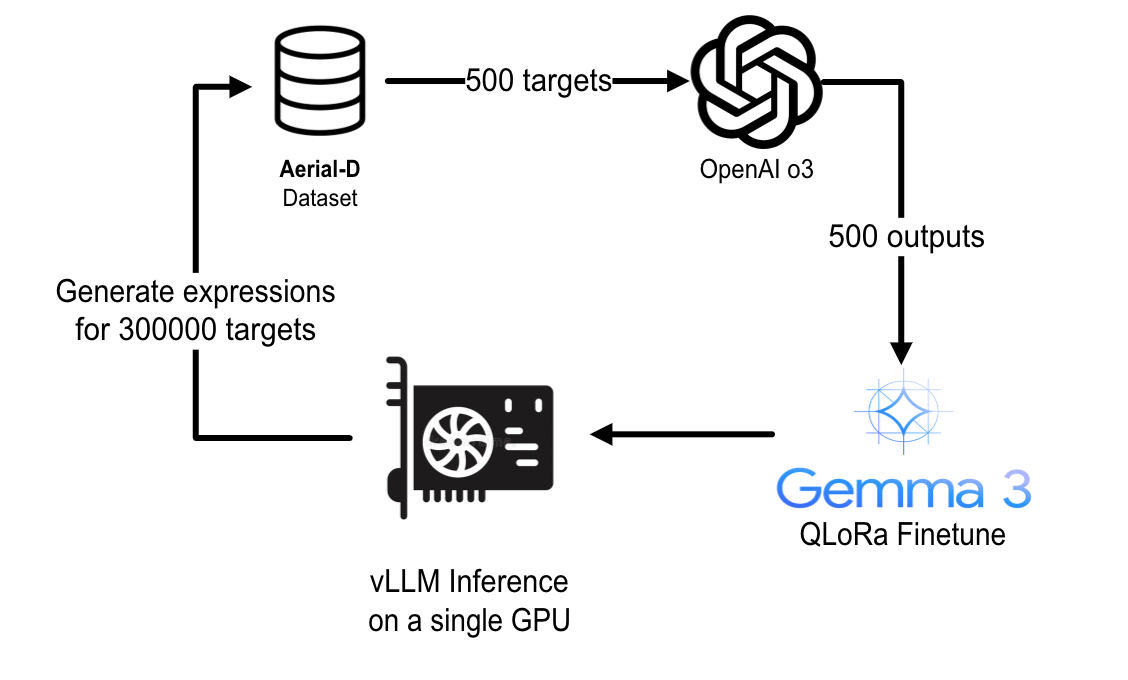
\includegraphics[width=\columnwidth]{./images/distillation.png}
\caption{Knowledge distillation pipeline for scalable LLM enhancement. A small sample of 500 expressions is processed through OpenAI's o3 model\cite{o3} to generate high-quality training targets, which are then used to fine-tune Gemma3‑12B\cite{gemma3} via QLoRA\cite{qlora}. The fine‑tuned model enables cost‑effective local inference to enhance the full dataset using vLLM\cite{vllm} on a single GPU.}
\label{fig:llm_distillation}
\end{figure}


%%%%%%%%%%%%%%%%%%%%%%%%%%%%%%%%%%%%%%%%%%%%%%%%%%%%%%%%%%%%%%%%%%%%%%
% EXPERIMENTS
%%%%%%%%%%%%%%%%%%%%%%%%%%%%%%%%%%%%%%%%%%%%%%%%%%%%%%%%%%%%%%%%%%%%%%
%%%%%%%%%%%%%%%%%%%%%%%%%%%%%%%%%%%%%%%%%%%%%%%%%%%%%%%%%%%%%%%%%%%%%%
%     File: ExtendedAbstract_resul.tex                               %
%     Tex Master: ExtendedAbstract.tex                               %
%%%%%%%%%%%%%%%%%%%%%%%%%%%%%%%%%%%%%%%%%%%%%%%%%%%%%%%%%%%%%%%%%%%%%%

\section{Experiments}
\label{sec:experiments}



%%%%%%%%%%%%%%%%%%%%%%%%%%%%%%%%%%%%%%%%%%%%%%%%%%%%%%%%%%%%%%%%%%%%%%
% CONCLUSION AND FUTURE WORK
%%%%%%%%%%%%%%%%%%%%%%%%%%%%%%%%%%%%%%%%%%%%%%%%%%%%%%%%%%%%%%%%%%%%%%
%%%%%%%%%%%%%%%%%%%%%%%%%%%%%%%%%%%%%%%%%%%%%%%%%%%%%%%%%%%%%%%%%%%%%%
%     File: ExtendedAbstract_concl.tex                               %
%     Tex Master: ExtendedAbstract.tex                               %
%%%%%%%%%%%%%%%%%%%%%%%%%%%%%%%%%%%%%%%%%%%%%%%%%%%%%%%%%%%%%%%%%%%%%%

\section{Conclusion and Future Work}
\label{sec:conclusion}

This work presents a comprehensive approach to open-vocabulary segmentation of aerial photographs through the development of AerialSeg and the AerialD dataset. By building upon the RSRefSeg architecture and implementing a systematic pipeline for dataset generation, we have demonstrated the feasibility of extending referring segmentation capabilities to the aerial domain.

Our rule-based annotation system successfully transforms existing semantic and instance segmentation datasets into rich referring segmentation resources, enabling the creation of natural language descriptions for objects in overhead imagery. The integration of spatial relationships, size comparisons, and color analysis provides a foundation for generating diverse and contextually relevant referring expressions that capture the unique characteristics of aerial scenes.

The enhancement of our dataset through large language models represents a significant advancement in dataset quality and diversity. By leveraging models such as Gemma3, we have shown that automatically generated referring expressions can be refined to achieve more natural and varied language patterns while maintaining semantic accuracy. This approach demonstrates the potential for scalable dataset creation that combines rule-based precision with the linguistic sophistication of modern language models.

Our experimental results validate the effectiveness of the RSRefSeg architecture when adapted to aerial imagery, showing promising performance on the task of open-vocabulary segmentation in overhead scenes. The combination of SigLIP and SAM backbones, enhanced through parameter-efficient LoRA fine-tuning, provides a robust foundation for handling the unique challenges of aerial image understanding.

\subsection{Future Work}

The field of open-vocabulary aerial image segmentation presents numerous opportunities for advancement, particularly through the integration of emerging multimodal technologies. A promising direction lies in leveraging new large language models that possess pixel-level segmentation capabilities, such as vision-language models with inherent understanding of spatial relationships and object boundaries.

These advanced models could serve dual purposes in future work. First, they could replace or augment the current RSRefSeg architecture as the base segmentation model, potentially offering more sophisticated understanding of the relationship between natural language descriptions and visual content. Their integrated approach to vision and language processing could eliminate the need for separate encoder architectures and complex fusion mechanisms.

Second, and perhaps more significantly, such models could revolutionize the dataset generation process itself. Beyond their current use for enhancing referring expressions, pixel-aware language models could generate entirely new segmentation masks based on textual descriptions, creating truly synthetic yet realistic aerial imagery datasets. This capability would enable the creation of datasets that are not constrained by the original annotations of existing semantic segmentation datasets, allowing for the generation of novel object configurations, rare scenarios, and specialized use cases that may be difficult to capture in real-world aerial photography.

This approach would make the segmentation system truly general in what it can segment, moving beyond the limitations of predefined object categories toward genuine open-vocabulary capabilities. The combination of advanced language models for both architecture and data generation could establish a new paradigm for aerial image understanding that is both more flexible and more comprehensive than current approaches.



%%%%%%%%%%%%%%%%%%%%%%%%%%%%%%%%%%%%%%%%%%%%%%%%%%%%%%%%%%%%%%%%%%%%%%
% REFERENCES
%%%%%%%%%%%%%%%%%%%%%%%%%%%%%%%%%%%%%%%%%%%%%%%%%%%%%%%%%%%%%%%%%%%%%%

% Produces the bibliography section when processed by BibTeX
%
% Bibliography style
% > entries ordered alphabetically
%\bibliographystyle{plain}
% > unsorted with entries appearing in the order in which the citations appear.
%\bibliographystyle{unsrt}
% > entries ordered alphabetically, with first names and names of journals and months abbreviated
\bibliographystyle{abbrv}
% > entries ordered alphabetically, with reference markers based on authors' initials and publication year
%\bibliographystyle{alpha}

% External bibliography database file in the BibTeX format (ExtendedAbstract_ref_db.bib)
\bibliography{ExtendedAbstract_ref_db}

%%%%%%%%%%%%%%%%%%%%%%%%%%%%%%%%%%%%%%%%%%%%%%%%%%%%%%%%%%%%%%%%%%%%%%
\end{document}
%%%%%%%%%%%%%%%%%%%%%%%%%%%%%%%%%%%%%%%%%%%%%%%%%%%%%%%%%%%%%%%%%%%%%%
